\documentclass{IEEEoj}
\usepackage{cite}
\usepackage{amsmath,amssymb,amsfonts}
\usepackage{algorithmic}
\usepackage{graphicx,color}
\usepackage{textcomp}
\def\BibTeX{{\rm B\kern-.05em{\sc i\kern-.025em b}\kern-.08em
    T\kern-.1667em\lower.7ex\hbox{E}\kern-.125emX}}
\def\OJlogo{\vspace{-10pt}
\includegraphics[height=20pt]{OJAP.png}}
\begin{document}
\receiveddate{XX Month, XXXX}
\reviseddate{XX Month, XXXX}
\accepteddate{XX Month, XXXX}
\publisheddate{XX Month, XXXX}
\currentdate{XX Month, XXXX}
\doiinfo{OJAP.2020.1234567}

\title{Ray-tracing Based RIS Size, Position and Target Points Optimization for Indoor Coverage Enhancement}

\author{EMRE KILCIOGLU, AND CLAUDE OESTGES}
\corresp{ICTEAM/ELEN, Universit\'e catholique de Louvain, Louvain-la-Neuve, Belgium\\\\
	CORRESPONDING AUTHOR: E. KILCIOGLU (e-mail: emre.kilcioglu@uclouvain.be)}
\authornote{This study was conducted as part of the project Win2Wal2023/1 - N°2310026 - RAFINE, funded by Région Wallonne.}
\markboth{Ray-tracing Based RIS Size, Position and Target Points Optimization for Indoor Coverage Enhancement}{Kilcioglu \textit{et al.}}

\begin{abstract}
....
\end{abstract}

\begin{IEEEkeywords}
......
\end{IEEEkeywords}

%\IEEEspecialpapernotice{(Invited Paper)}

\maketitle

\section{INTRODUCTION}
\IEEEPARstart{T}{his} .....

\section{RIS MODELING}
This section describes how the RIS is represented and incorporated within the ray-tracing simulation tool, specifically NVIDIA's Sionna RT \cite{sionna}. The RIS is strategically positioned to ensure line-of-sight (LoS) connectivity with both the transmitter and the designated target positions. These target positions typically correspond to blind zones in the transmitter-only coverage, where direct signal reception is either weak or entirely obstructed. By utilizing the RIS, reflected signals can be directed into these blind zones, enhancing overall system coverage and performance.

The RIS surface is discretized into a grid of \(N \times M\) tiles, each defined by the discretization sizes \(d_y\) and \(d_z\), as illustrated in Fig. \ref{RIS_Modeling}. Each tile, denoted as \(T_{n,m}\) for the \(n^{\text{th}}\) row and \(m^{\text{th}}\) column, is characterized by a complex reflection coefficient. These coefficients govern the phase and amplitude adjustments applied to incident electromagnetic waves. By choosing sufficiently small discretization sizes, the RIS surface can effectively approximate a continuous surface, enabling a high degree of control over the reflected wavefronts. Without loss of generality, the RIS is assumed to be aligned within the y-z plane of the 3D simulation environment.

The functionality of the RIS is governed by the combined contributions of all tiles, which collectively direct the reflected signals toward \(K \geq 1\) predefined target positions. For simplicity, Fig. \ref{RIS_Modeling} depicts only one target position. The complex reflection coefficient of a single tile is mathematically expressed as:
\[
\Gamma_{n,m} = \sum \limits_{k=1}^K \sqrt{c_k} A_{n,m}^k e^{j \varphi_{n,m}^k},
\]
where \(A_{n,m}^k\) and \(\varphi_{n,m}^k\) represent the amplitude and phase adjustments, respectively, for the \(k^{\text{th}}\) target position. These coefficients form the 2D profiles of reflection amplitude \(\mathbf{A}^k\), phase \(\mathbf{\Phi}^k\), and the overall reflection coefficient \(\mathbf{\Gamma}\) for the RIS. The power intensity coefficient \(c_k\), which determines the proportion of the RIS's reflection energy allocated to the \(k^{\text{th}}\) target position, satisfies the normalization constraint:
\[
\sum_{k=1}^K c_k = 1.
\]

The proposed RIS modeling approach is highly versatile and allows for simulating various RIS configurations under diverse environmental conditions. For instance, in complex indoor environments with significant obstructions, such as walls or large furniture, the RIS can mitigate coverage gaps by intelligently reflecting incident signals into otherwise unreachable areas. By carefully designing the amplitude and phase profiles of the RIS, signals can be steered around obstacles, overcoming shadowing effects and enhancing the received signal power in designated regions.

Moreover, the granularity of the RIS discretization provides flexibility in achieving different reflection patterns. For example, smaller discretization sizes yield finer control over the reflected wavefronts, enabling higher precision in focusing or beam-steering tasks. These capabilities make the RIS a powerful tool for addressing a wide range of propagation challenges, including non-line-of-sight (NLoS) scenarios and dynamic coverage enhancement requirements.

\begin{figure}
	\centering 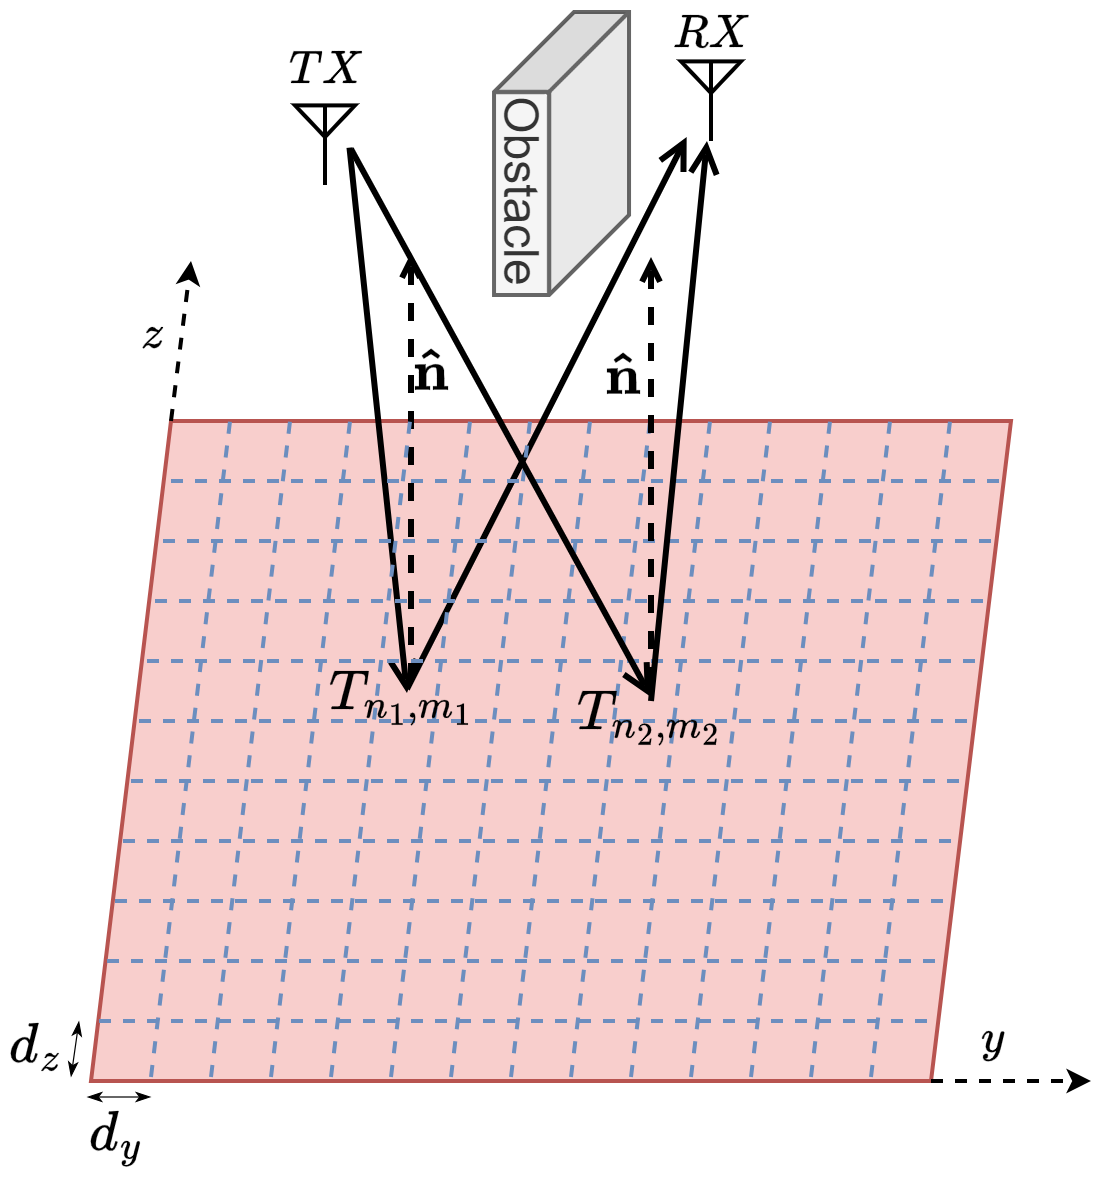
\includegraphics[width=.62\linewidth]{RIS_Modeling.png}
	\caption{Illustration of RIS modeling: The RIS surface is discretized into tiles, each with tunable reflection characteristics, to direct signals toward target positions.}
	\label{RIS_Modeling}
	\vspace{-0.5cm}
\end{figure}

This detailed modeling framework, implemented in Sionna RT, provides a robust foundation for exploring the potential of RIS in improving wireless communication performance. By leveraging this model, we can systematically evaluate the impact of different RIS configurations and optimization strategies, including those introduced in this study, to address coverage challenges in both static and dynamic environments.

\section{PHASE PROFILE ASSIGNMENT APPROACHES}
In this section, we discuss two primary approaches for assigning the phase profiles to the RIS to achieve anomalous reflections for each target position \( k \). These methods are the \textbf{gradient-based} \cite{phase_grad_paper} and \textbf{distance-based} \cite{Tang} approaches. Both approaches offer distinct advantages, making them suitable for different scenarios and environmental conditions.

\begin{enumerate}
	\item \textbf{Gradient-Based Approach}: This method considers the incidence and desired reflection wave directions, and it aims to achieve the desired reflection direction by introducing a phase gradient across the RIS surface. The phase gradient is computed to align the reflected signal with the desired reflection direction, thereby optimizing the coverage at the target positions.
	
	\item \textbf{Distance-Based Approach}: In contrast to the gradient-based method, the distance-based approach focuses on the total distance traveled by the incident and reflected signals. By adjusting the phase shifts to match the distances from the transmitter to each tile and from each tile to the target positions, the method ensures that the reflected signals constructively interfere at the target positions.
\end{enumerate}

The phase profile for these approaches is calculated for each target position \( k \), and the individual phase profiles are combined through the summation in (\ref{ref_coef_exp}) to derive the final reflection coefficient profile \( \mathbf{\Gamma} \). To simplify the notation, the parameters related to target positions are expressed without the index \( k \) during the intermediate calculations, although the profiles inherently depend on \( k \).

\subsection{GRADIENT-BASED PHASE PROFILE}
The gradient-based approach, as illustrated in Fig. \ref{RIS_Phase_Gradient}, treats the RIS as an ideal phase gradient reflector. The phase gradient is calculated based on the incident wave direction and the desired reflection direction for each target position. In this method, the RIS introduces a phase gradient that modifies the direction of the reflected waves, aiming to direct the reflected signal toward the target position.

Let us consider an incident wave with wave vector \( \mathbf{\hat{k}}_i \) arriving at the center of the RIS at an incidence angle \( \theta_i \) with respect to the RIS normal vector \( \mathbf{\hat{n}} \). The desired reflection for the target position \( k \) is represented by the reflection wave vector \( \mathbf{\hat{k}}_r \), with reflection angle \( \theta_r \). The incident phase gradient due to the inclined wavefront is given by:
\[
\nabla \varphi_i = - k_0 \sin\theta_i \, \mathbf{\hat{k}}_i^p = - k_0 \, \textbf{P} \mathbf{\hat{k}}_i,
\]
where \( k_0 = 2 \pi / \lambda \) is the wavenumber and \( \lambda \) is the wavelength. Here, \( \mathbf{\hat{k}}_i^p \) represents the unit projection vector of the incident wave vector onto the RIS, and \( \textbf{P} \) is the projection operator, where \( \textbf{P} \mathbf{\hat{k}}_i = \sin\theta_i \, \mathbf{\hat{k}}_i^p \).

The RIS applies an additional phase gradient \( \nabla \varphi_{RIS} \), such that the total reflection phase gradient \( \nabla \varphi_r \) is:
\[
\nabla \varphi_r = \nabla \varphi_i + \nabla \varphi_{RIS}.
\]
Similarly to the incident wave, the reflection phase gradient \( \nabla \varphi_r \) is expressed as:
\[
\nabla \varphi_r = - k_0 \sin\theta_r \, \mathbf{\hat{k}}_r^p = - k_0 \, \textbf{P} \mathbf{\hat{k}}_r,
\]
where \( \mathbf{\hat{k}}_r^p \) is the unit projection vector of the reflection wave vector \( \mathbf{\hat{k}}_r \) onto the RIS. By substituting (\ref{grad_phi_i}) and (\ref{grad_phi_r}) into the expression for the total phase gradient, we find the desired phase gradient on the RIS:
\[
\nabla \varphi_{RIS} = k_0 \, \textbf{P} (\mathbf{\hat{k}}_i - \mathbf{\hat{k}}_r) = k_0 \, (\sin\theta_i \, \mathbf{\hat{k}}_i^p - \sin\theta_r \, \mathbf{\hat{k}}_r^p).
\]
This phase gradient drives the reflection of signals toward the target position. For simpler cases, such as when the RIS, transmitter, and target positions are at the same height, the gradient becomes one-dimensional along the y-axis:
\[
\nabla \varphi_{RIS} = k_0 \, (\sin\theta_i - \sin\theta_r) \, \hat{y}.
\]
This simplification results in a one-dimensional phase gradient and a more straightforward implementation of the RIS design.

The phase profile \( \mathbf{\Phi}^k \) for each target position \( k \) is then generated by setting the first RIS tile phase to zero and applying a linear variation of the phase across the tiles, following the gradient calculated in (\ref{grad_exp}).

\begin{figure}
	\centering 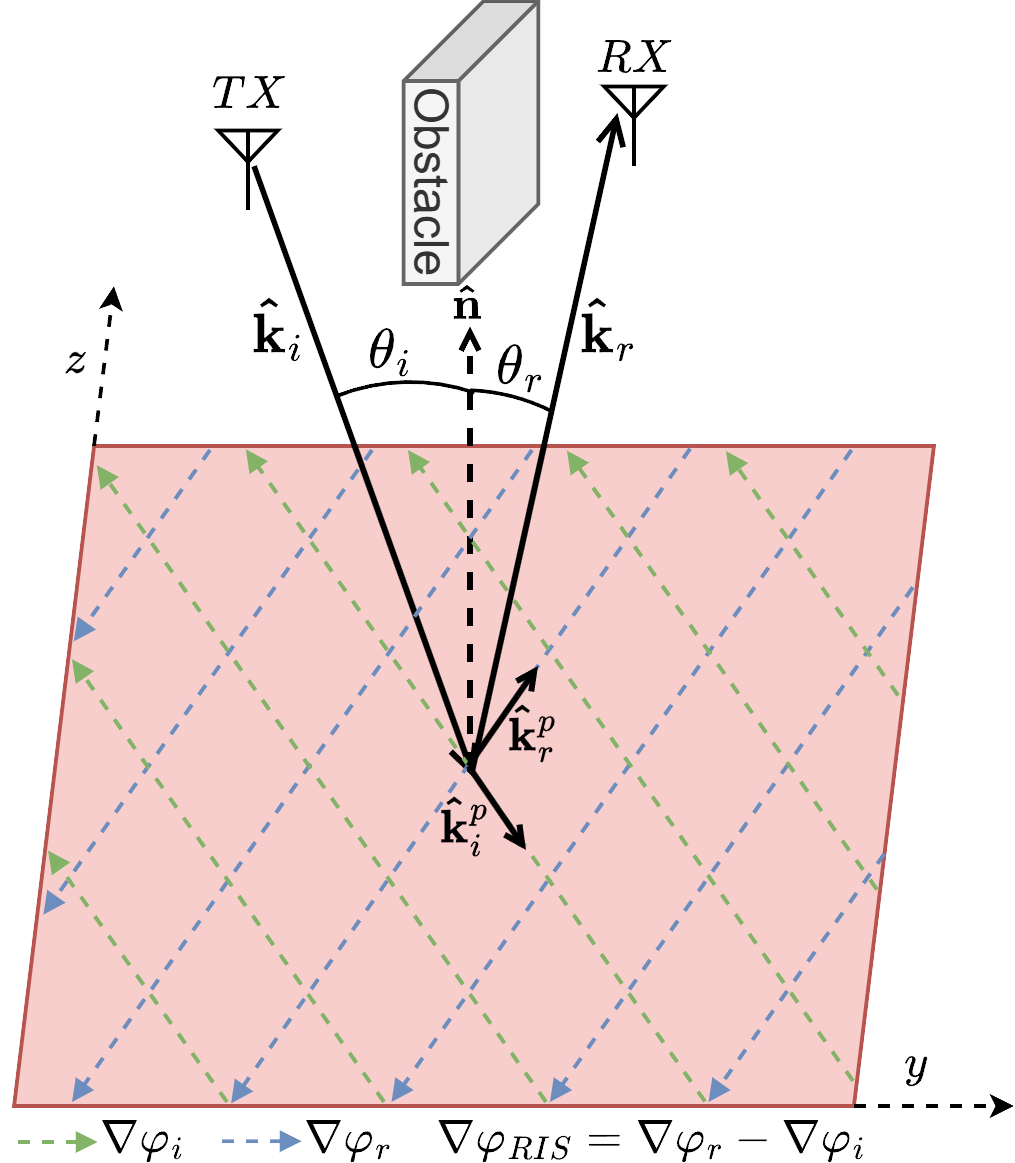
\includegraphics[width=.87\linewidth]{RIS_Phase_Gradient.png}
	\caption{Illustration of the gradient-based RIS approach, where the RIS applies a phase gradient to control the reflection direction.}
	\label{RIS_Phase_Gradient}
\end{figure}

\subsection{DISTANCE-BASED PHASE PROFILE}
The distance-based approach models the RIS as a focusing lens that ensures the reflected signals from all tiles combine coherently at the target position. In this method, the phase shift for each tile is determined by the total distance traveled by the signal from the transmitter to the tile and from the tile to the target position.

The position of each tile \( T_{n,m} \) relative to the RIS center is given by:
\[
(0, (m-\frac{1}{2})d_y, (n-\frac{1}{2})d_z),
\]
where \( m \in \left[ 1 - \frac{M}{2}, \frac{M}{2} \right] \) and \( n \in \left[ 1 - \frac{N}{2}, \frac{N}{2} \right] \) represent the row and column indices of the tile.

The electric field arriving at each tile \( T_{n,m} \) is expressed as:
\[
E_{n,m}^{\text{in}} = \sqrt{\frac{2 Z_0 P_{n,m}^{\text{TX-RIS}}}{d_y d_z}} e^{-j \frac{2 \pi r_{n,m}^{tx}}{\lambda}},
\]
where \( Z_0 \) is the characteristic impedance of free space, \( r_{n,m}^{tx} \) is the distance between the transmitter and \( T_{n,m} \), and \( P_{n,m}^{\text{TX-RIS}} \) is the received power at each tile. After reflection, the total electric field at the target position \( k \) is:
\[
E^{rx} = \sum_{n=-\frac{N}{2}}^{\frac{N}{2}} \sum_{m=-\frac{M}{2}}^{\frac{M}{2}} E_{n,m}^{rx}.
\]

Each reflected field at tile \( T_{n,m} \) is:
\[
E_{n,m}^{rx} = \sqrt{\frac{2 Z_0 P^{rx}_{n,m}}{A_{rx}}} e^{-j \left( \frac{2 \pi}{\lambda} \left( r_{n,m}^{tx} + r_{n,m}^{rx} \right) - \varphi_{n,m}^k \right)},
\]
where \( r_{n,m}^{rx} \) is the distance from tile \( T_{n,m} \) to the receiver, \( A_{rx} \) is the receiving antenna aperture, and \( P_{n,m}^{rx} \) is the power of the reflected signal at target position \( k \).

The received power at target position \( k \) is then given by:
\[
P^{rx} = \frac{\left| E^{rx} \right|^2}{2 Z_0} A_{rx} = \left| \sum_{n=-\frac{N}{2}}^{\frac{N}{2}} \sum_{m=-\frac{M}{2}}^{\frac{M}{2}} A_{n,m}^k \sqrt{P_{n,m}^{\text{TX-RIS}} P_{n,m}^{\text{RIS-RX}}} e^{-j \left( \frac{2 \pi}{\lambda} \left( r_{n,m}^{tx} + r_{n,m}^{rx} \right) - \varphi_{n,m}^k \right)} \right|^2.
\]

Maximizing the received power leads to the condition:
\[
\varphi_{n,m}^k = \frac{2 \pi}{\lambda} \left( r_{n,m}^{tx} + r_{n,m}^{rx} \right),
\]
which is the phase profile that must be assigned to each tile to achieve constructive interference at the target position \( k \).


\begin{IEEEbiography}[{
\includegraphics[width=1in,height=1.25in,clip,keepaspectratio]{Emre_Picture.jpg}}]{EMRE KILCIOGLU } received his B.Sc. and M.Sc. degrees in Electrical and Electronics Engineering from Middle East Technical University, Ankara, Turkey, in 2016 and 2019, respectively. He completed his Ph.D. in 2024 at the Institute of Information and Communication Technologies, Electronics and Applied Mathematics (ICTEAM), Université catholique de Louvain (UCLouvain), Louvain-la-Neuve, Belgium, where he is currently a postdoctoral researcher.
	
From July 2016 to January 2020, he worked as a system design engineer at Aselsan Inc., Ankara, Turkey. His research interests include massive MIMO, cooperative communication, deep learning applications in wireless communications, and ray-tracing-based optimization of reconfigurable intelligent surfaces (RISs).
\end{IEEEbiography}

\begin{IEEEbiography}[{
\includegraphics[width=1in,height=1.25in,clip,keepaspectratio]{Emre_Picture.jpg}}]{CLAUDE OESTGES } ...
\end{IEEEbiography}

\end{document}
